\documentclass{article}
\usepackage{tabularx}
\usepackage{amsmath}
\usepackage{graphicx}
\usepackage[top = 2cm, bottom = 2cm, right = 2cm, left = 2cm]{geometry}
\usepackage{cite}
\usepackage[final]{hyperref}
\usepackage{listings}
\hypersetup{
	colorlinks=true,
	linkcolor=blue,
	citecolor=blue,
	filecolor=magenta,
	urlcolor=blue         
}

\begin{document}

\title{Practicle 3\\Raytracer - Ray}
\date{16/01/19}
\maketitle

\begin{abstract}
	On this practical work we will learn how to send ray from a camera through a screen. To do this, we need to understand the different screen spaces.
\end{abstract}

\section{The \_\_host\_\_ key word}
We sent in the last practical a kernel to clear the background color of our image. We use two versions of the same class and we cast the parameter when we pass the argument. The keyword \_\_host\_\_ allow us to declare a function on the host. Fortunately it can be combined with the \_\_device\_\_ keyword. 
\begin{lstlisting}
	__host__ __device__ void foo();
\end{lstlisting}
The function foo can be called from both the host and the device. You can use this keyword to avoid the Vector3 code duplication. However you have to be careful because some standard function can have different behaviours. For example CUDA use the IEEE 754 standard, you have to be sure your host use the same.\\

\section{The UV coordinate}
Currently, we use image as a linear buffer. But, to send ray we need to use the uv coordinate system. It is a vector space with two dimension from 0 to 1. Let's see how to convert our linear index to the uv paradigm. Fisrt, we need another kernel to compute the x and y pixel coordinate from the index. 
\begin{lstlisting}
	unsigned int x = i%h;
	unsigned int y = i/h;
\end{lstlisting}
After a floating conversion we can divide x by the width to get the u value. Do the same for v.\\
To be sure u and v are correctly computed we can show them. The problem in graphic computing is debugging. Because it's not host code we cannot use breakpoint from the IDE. We'll see how CUDA can be debugged and profiled in the parctical 5.\\
Because are between 0 and 1 we can use them as color. 
\begin{lstlisting}
	image[i] = Vector3(u, v, 0.f);
\end{lstlisting}
\begin{figure}[h]
	\centering
	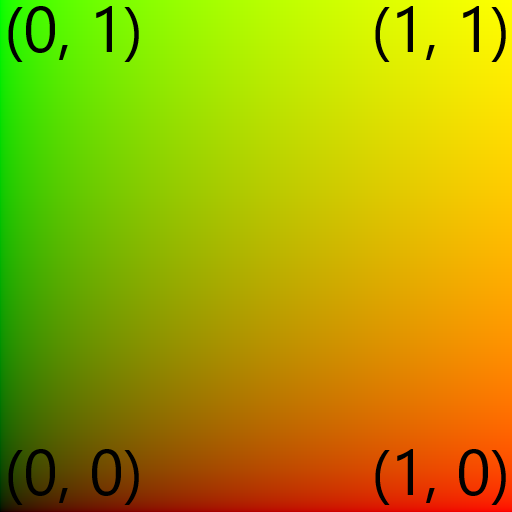
\includegraphics[scale=0.2]{figures/uv.png}
	\caption{UV}
\end{figure}
By the way, most of the image of this website (https://www.shadertoy.com/) are computed with only uv coordinate.

\section{Send ray}
As expected, rays are the most important part of a raytracer. It's just an origin point and a direction. Create a class for instantiate a ray in a kernel and provide a function to compute a point on the ray ($P = Origin + Direction*t$).\\
We'll send one ray per pixel from a camera. At this point you have two options. You can generate your rays:
\begin{itemize}
	\item from each pixel with a perpendicular direction to the screen (orthogonal view)
	\item from an origin point to each pixel of the screen (persepective view)
\end{itemize}
The second option is the most common for a ray tracer. We need a camera at the origin $O = (0, 0, 0)$ and a screen in front of the camera $(0, 0, -1)$. Because the first pixel of the image is not on the center of the screen we need to translate it. So the left lower corner ($L$) is $L = (-0.5, -0.5, -1) = (0, 0, -1) - (0.5, 0.5, 0)$. Adding uv coordinate to the left lower corner give the 3D pixel coordinate ($P$). $P = L + (u, v, 0)$. Finally, our ray is \{$origin=O | direction=P-O$\}
\begin{figure}[h]
	\centering
	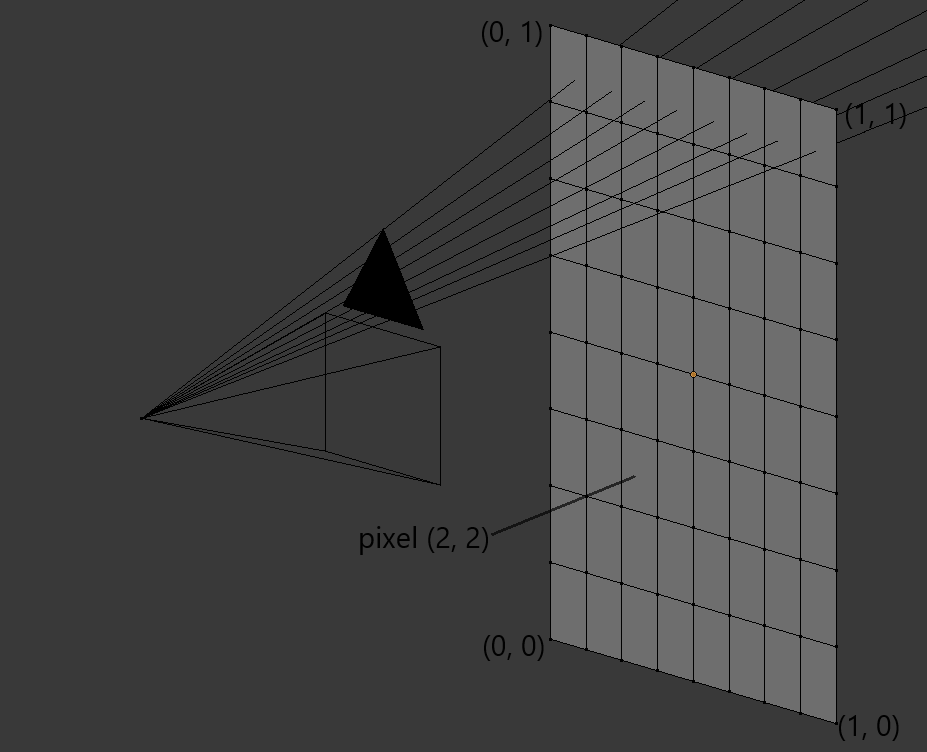
\includegraphics[scale=0.5]{figures/screen.png}
	\caption{UV}
\end{figure}
When we write some heavy algorithm there is often error due to call stack size too small or to much thread ran per block. To be sure the program going well we can use cudaGetLastError at the end.
\begin{lstlisting}
	cudaError_t err = cudaGetLastError();
	if (err != cudaSuccess) printf("%s\n", cudaGetErrorString(err));
\end{lstlisting}

\end{document}